\chapter{sPHENIX overview}
\label{chap:introduction}
\section{Science mission}
Over the last decades, experiments at RHIC and LHC have shown that collisions of heavy nuclei produce a novel hot and dense state of matter, called Quark-Gluon Plasma (QGP). These studies demonstrated that the QGP has properties that are unique among all forms of matter - in particular it is the most perfect liquid known. The QGP is a key example of a class of strongly coupled systems found recently in wide range of areas of physics, from string theory to condensed matter and ultra-cold atom systems.

While measurements have provided detailed knowledge of the QGP's macroscopic (long wavelength) properties, we do not yet understand how these properties arise from the fundamental interactions of its constituents, i.e., quarks and gluons governed by the laws of Quantum Chromodynamics (QCD).  In the 2015 Hot QCD Whitepaper and the US Nuclear Physics Long Range Plan (LRP)~\cite{Geesaman:2015fha}, one of two highest  priority goals in the field of Hot QCD was described as ``Probe the inner workings of QGP by resolving its properties at shorter and shorter length scales. The complementarity of the two facilities i.e., [RHIC and LHC] is essential to this goal, as is a state-of-the-art jet detector at RHIC, called sPHENIX''~\cite{Geesaman:2015fha}.

\begin{figure}[htpb]
\begin{center}
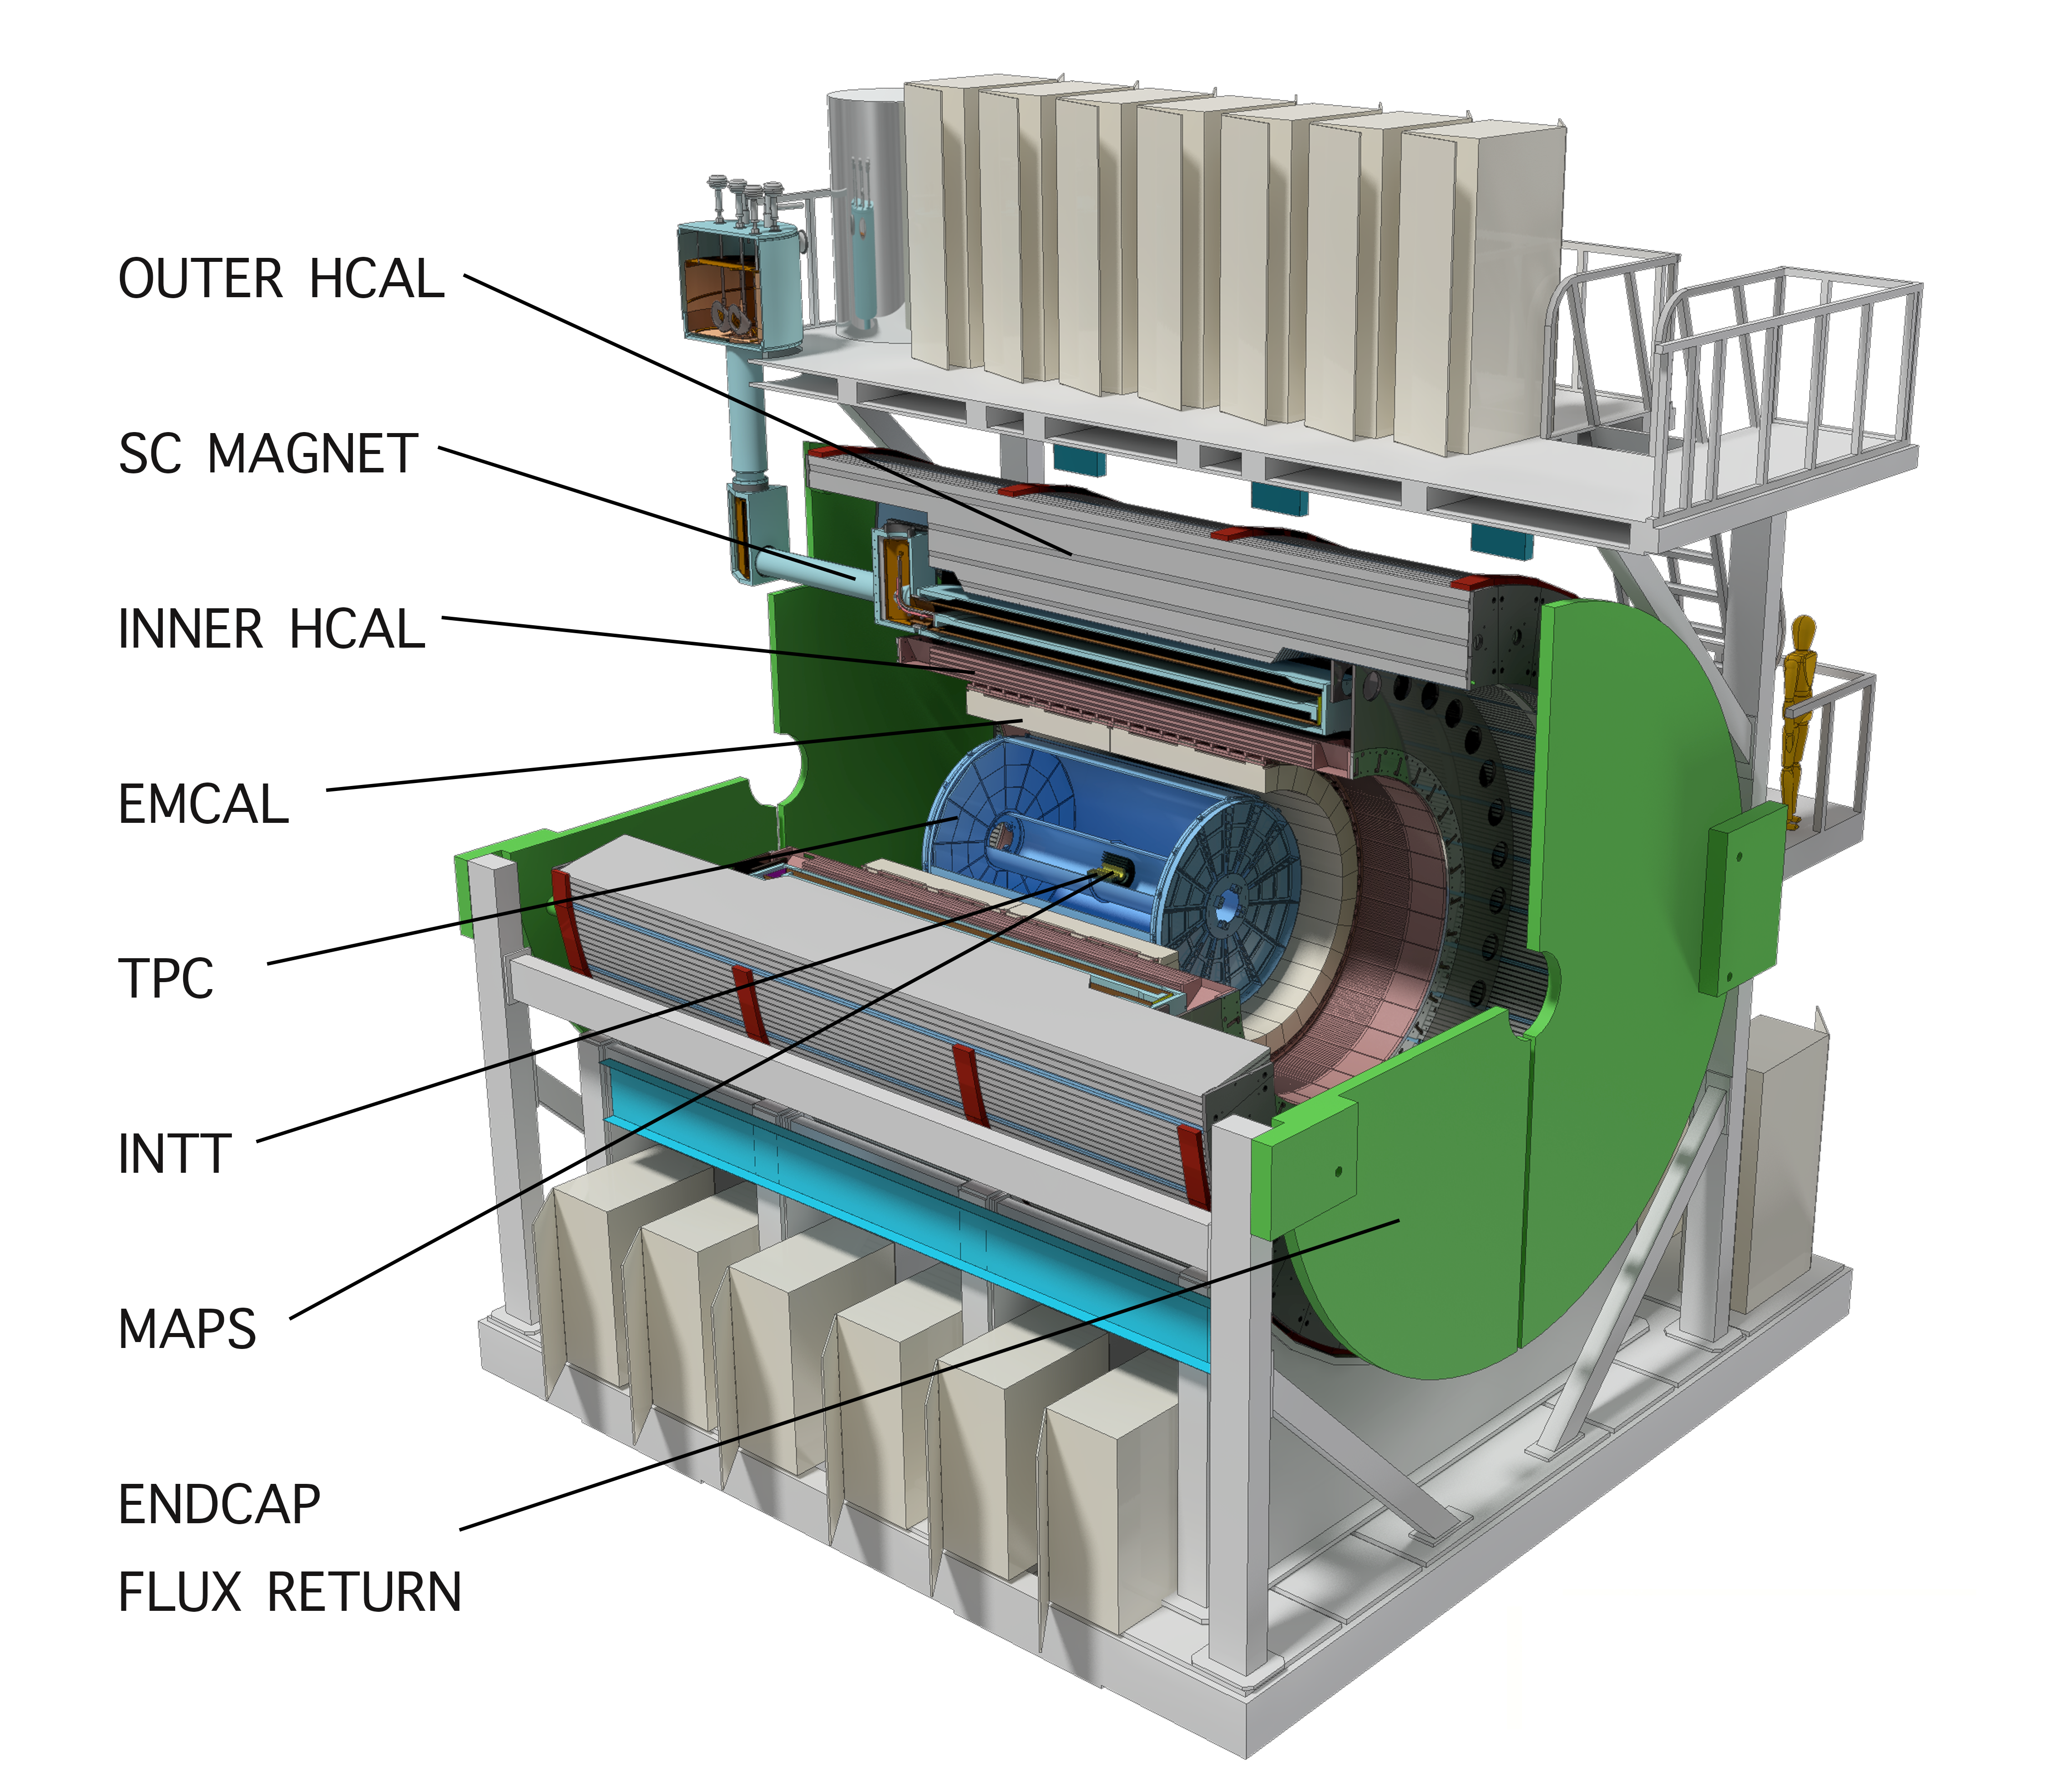
\includegraphics[width=0.8\textwidth]{figs/sPhenix-Assembly-Labeled-With-Tracking-Shaded_with_Black_Lines-3600-BRIG.png}
\end{center}
\vspace{-0.5cm}
\caption{\label{fig:sPHENIX} Engineering drawing (cutaway) of the
  sPHENIX detector. From the inside out the drawing shows tracking
  system, electromagnetic calorimeter and inner hadronic calorimeter,
  superconducting magnet and outer hadronic calorimeter.  Although
  PHENIX was more than twice as heavy as sPHENIX, its larger mass was
  distributed across four different movable carriages.  The supporting
  rail system will be reinforced with high strength concrete to
  provide an appropriate safety margin for the sPHENIX carriage. A
  detailed discussion of the sPHENIX detector subsytems can be found
  in the sPHENIX Technical Design Report~\cite{sPHENIX:TDR}}
\end{figure}

To elucidate the nature of the QGP, the sPHENIX physics program rests on a broad set of measurements using hard probes that are sensitive to the QGP microscopic structure over a range of length or momentum scales. These measurements include in particular studies of jet production and substructure, quarkonia suppression and open heavy flavor production and correlations. The sPHENIX studies will complement those planned at LHC for Run 3 during high luminosity Pb+Pb operations and provide qualitative improvements over current measurements at RHIC for related observables.

sPHENIX was proposed by the PHENIX collaboration in their 2010 decadal plan as an upgrade (or replacement) of the PHENIX experiment at RHIC. The physics case and detector design were further developed in the years leading up to the 2015 Nuclear Physics LRP. A detailed design proposal was completed in 2015~\cite{sPHENIX:2015irh}, and in early 2016 the current sPHENIX collaboration was formed. As of early 2020, sPHENIX has more than 320 members from 80 institutions in 13 countries. The project received DOE CD-0 approval in late 2016, CD-1/3A approval in 2018 and entered its construction phase after PD 2/3 approval in fall 2019. The current schedule foresees commissioning of the detector in 2022 and start of physics data taking in early 2023. The current expectations for 2025 as the final year of sPHENIX operations is dictated by BNL's reference schedule for the EIC project.

\section{sPHENIX performance measures}

sPHENIX has been designed to allow high-statistics, high-resolution measurements for a broad
range of observables related to jet production and modification, quarkonia production
at high mass (or high \pt) and yields and correlations of heavy quark (charm \em and \em bottom) hadrons and heavy flavor tagged jets.
This is achieved through several advances compared to the current instrumentation at RHIC:
\begin{itemize}
    \item The sPHENIX tracking and calorimetry provide hermetic coverage over full azimuth and pseudorapidity $|\eta| < 1$, with a readout rate of 15~kHz for all subdetectors. The detector also provides triggering capabilities in \pp, and for selected observables in \aa, as well as the option for streaming readout of the tracking detectors. In combination, statistical precision compared to the current status at RHIC will improve  by 1-2 orders of magnitude for many observables.
    \item The MAPS-based MVTX micro-vertex detector provides larger acceptance, faster readout and higher resolution compared to previous RHIC detectors, enabling a state-of-the-art open heavy flavor program, including a large set of b-hadron measurements. 
    \item As a first at RHIC, sPHENIX features large acceptance hadronic calorimetry, enabling unbiased selection (and triggering in \pp) for jets, as well as improving jet resolution and extending the range for high \pt single hadron measurements through rejection of misreconstructed tracks. In combination with the MVTX, this will alllow the first application of b-jet tagging at RHIC. 
\end{itemize}
Various benchmark plots for planned physics
measurements are shown in section~\ref{chap:physics_projections}. These projections are based on the expected statistics in the run plan described in this document and the detector performance and acceptance obtained from GEANT simulations.

The gains resulting from the sPHENIX rate capability and resolution are illustrated by kinematic range for single particle observables, relative to prior measurements at RHIC.
Figure~\ref{fig:sPHENIX_MIE_master_AuAu_projections_tshirtcompare} compares
statistical projections for sPHENIX for various observables after the first sPHENIX data
taking campaign to the corresponding current $R_\mathrm{AA}$ measurements in central
Au$+$Au events by the PHENIX Collaboration.
While the existing measurements have greatly contributed to our
understanding of the QGP created at RHIC, the overall kinematic reach is
constrained to $< 20$~GeV even for the highest statistics
measurements. In contrast, the projected sPHENIX measurements reach sufficiently high \pt to
provide a large overlap with both low and and high \pt measurements at the LHC.

